\documentclass[preprint, 3p,
authoryear]{elsarticle} %review=doublespace preprint=single 5p=2 column
%%% Begin My package additions %%%%%%%%%%%%%%%%%%%

\usepackage[hyphens]{url}

  \journal{Sustainable Cities and Society} % Sets Journal name

\usepackage{graphicx}
%%%%%%%%%%%%%%%% end my additions to header

\usepackage[T1]{fontenc}
\usepackage{lmodern}
\usepackage{amssymb,amsmath}
% TODO: Currently lineno needs to be loaded after amsmath because of conflict
% https://github.com/latex-lineno/lineno/issues/5
\usepackage{lineno} % add
\usepackage{ifxetex,ifluatex}
\usepackage{fixltx2e} % provides \textsubscript
% use upquote if available, for straight quotes in verbatim environments
\IfFileExists{upquote.sty}{\usepackage{upquote}}{}
\ifnum 0\ifxetex 1\fi\ifluatex 1\fi=0 % if pdftex
  \usepackage[utf8]{inputenc}
\else % if luatex or xelatex
  \usepackage{fontspec}
  \ifxetex
    \usepackage{xltxtra,xunicode}
  \fi
  \defaultfontfeatures{Mapping=tex-text,Scale=MatchLowercase}
  \newcommand{\euro}{€}
\fi
% use microtype if available
\IfFileExists{microtype.sty}{\usepackage{microtype}}{}
\usepackage[]{natbib}
\bibliographystyle{plainnat}

\usepackage{graphicx}
\ifxetex
  \usepackage[setpagesize=false, % page size defined by xetex
              unicode=false, % unicode breaks when used with xetex
              xetex]{hyperref}
\else
  \usepackage[unicode=true]{hyperref}
\fi
\hypersetup{breaklinks=true,
            bookmarks=true,
            pdfauthor={},
            pdftitle={Which fifteen-minutes neighborhoods are dead-ends? An analysis of the network attributes of fifteen-minute pedsheds},
            colorlinks=false,
            urlcolor=blue,
            linkcolor=magenta,
            pdfborder={0 0 0}}

\setcounter{secnumdepth}{5}
% Pandoc toggle for numbering sections (defaults to be off)


% tightlist command for lists without linebreak
\providecommand{\tightlist}{%
  \setlength{\itemsep}{0pt}\setlength{\parskip}{0pt}}







\begin{document}


\begin{frontmatter}

  \title{Which fifteen-minutes neighborhoods are dead-ends? An analysis
of the network attributes of fifteen-minute pedsheds}
    \author[University One]{Author One%
  \corref{cor1}%
  \fnref{1}}
   \ead{a1@example.com} 
    \author[University Two]{Author Two%
  %
  }
   \ead{a2@example.com} 
    \author[University One]{Author Three%
  %
  \fnref{2}}
   \ead{a3@example.com} 
    \author[University One]{Author Four%
  %
  \fnref{2}}
   \ead{a4@example.com} 
      \affiliation[University One]{
    organization={Department},addressline={1 main
street},city={City},postcode={123456},state={State},country={Country},}
    \affiliation[University Two]{
    organization={Department},addressline={2 main
street},city={City},postcode={2054},country={Country},}
    \cortext[cor1]{Corresponding author}
    \fntext[1]{This is the first author footnote.}
    \fntext[2]{Another author footnote.}
  
  \begin{abstract}
  Fifteen-minutes neihborhoods, a form of normative chronourbanism based
  on cumulative opportunities, has aroused interest as a way to reduce
  the need for motorized travel, and increase the livability,
  convenience, and health of the public. At the core of this concept is
  a pedshed, an area defined by the walkable isochrone of the eponymous
  fifteen minutes. As the idea of fifteen-minutes neighborhoods develops
  traction in policy and planning circles, it seems timely to revisit
  the way street network design can support---or obstruct---the stated
  goal of preserving or creating walkable neighborhoods with essential
  amenities. In this paper we examine a sample (\(n=834\)) of
  fifteen-minutes pedsheds in Hamilton, a medium-sized city in Canada,
  and how their sizes relate to the attributes of the transportation
  network. The analysis reveals that network design in suburban Hamilton
  conspires against the creating of fifteen-minutes neighborhoods. Much
  of urban Hamilton, in contrast, already has the characteristics of
  fifteen-minutes neighborhoods. The research points to elements of
  network design that can help to discriminate between candidate
  neighborhoods and dead-ends, and that can provide parameters for the
  design of new developments.
  \end{abstract}
    \begin{keyword}
    Fifteen-minutes
neighborhoods \sep Pedshed \sep Walkability \sep Accessibility \sep 
    Network analysis
  \end{keyword}
  
 \end{frontmatter}

The aim is to train a classification tree to profile urban and suburban
walksheds based on the attributes of the network. We need to drop 1
observation that has an NA in \texttt{transitivity}:

\begin{verbatim}
## pred
##   0   1 
## 114 228
\end{verbatim}

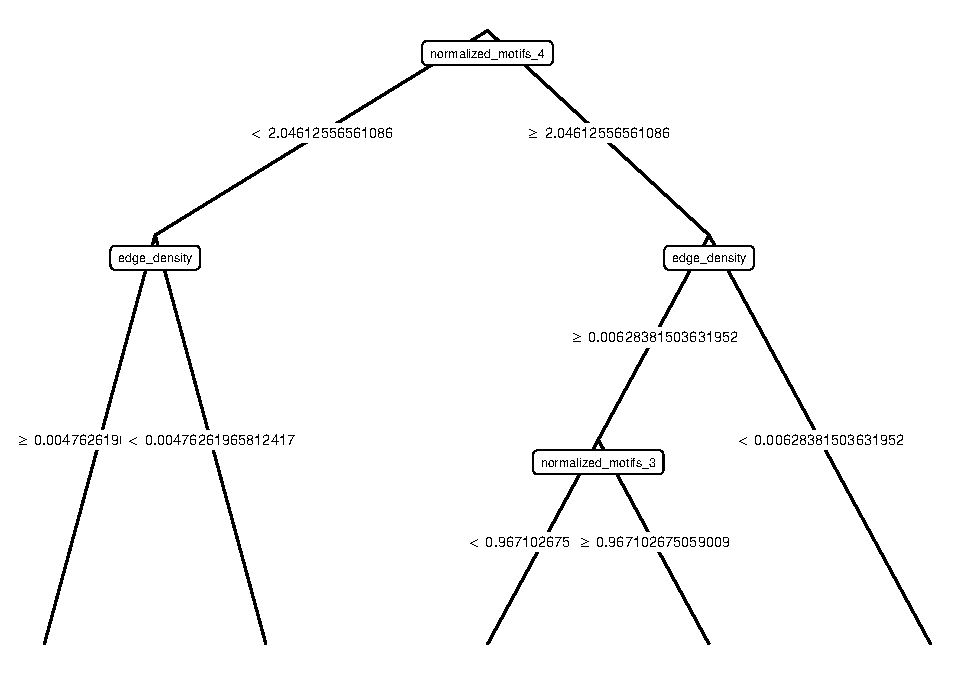
\includegraphics{paper_files/figure-latex/unnamed-chunk-3-1.pdf}

\section{Introduction}\label{introduction}

\begin{quote}
``Il faut oublier la traversée de Paris d'est en ouest en
voiture''\footnote{ ``We must forget about crossing Paris from east to
  west by car''}. --Anne Hidalgo
\end{quote}

With this declaration during her reelection campaign in 2020, Anne
Hidalgo brought international attention to the concept of walkable
fifteen-minutes neighborhoods \citep{alimi2020}.

\citet{knight2018walkable} \citet{liu2022toward}
\citet{pozoukidou2021fifteen} \citet{weng2019fifteen}

15-minute walking neighborhoods are studied, and their accessibility
levels assessed (positive analysis). Optimal opportunity landscapes are
then used to simulate equivalent opportunity landscapes throughout the
region. Accessibility is then reanalyzed from the normative perspective
of the provision of opportunities. The results of this analysis are
finally correlated to neighborhood network attributes, including
connectivity, centrality, and clustering

\section{Data}\label{data}

The data used to study 15-minute walking neighborhoods in the city of
Hamilton was obtained by extracting relevant attributes of the street
network within 15-minute pedestrian sheds. These sheds were calculated
for each neighborhood as polygon representations of origin-destination
walking time matrices, with a maximum travel time of 15 minutes.
Walkshed calculations were generated using the travel\_time\_matrix
function for walking from the \{r5r\} R package. This process involved
defining the street network, as well as the origins and destinations of
walking trips. The street network data for these calculations was
sourced from OpenStreetMap \citet{OpenStreetMap2023}.

The origins we established are proxies for the centroids of
neighborhoods in the urban and peri-urban areas of the city of Hamilton.
Specifically, these are the centroids of Hamilton's Dissemination Areas
(DA). A DA is composed of one or more neighboring dissemination blocks
and represents the smallest standard geographic area for which all
census data are disseminated in Canada. Data on urban and sub-urban
boundaries and DAs were retrieved from \citet{HamiltonData2023}.

Destinations were established as the centroids of geohashed hexagons
within the region of interest, where Hamilton's amenities are located,
assuming that presence of amenities is a proxy to provision of
opportunities. These destinations were chosen to avoid calculating
travel times to each individual amenity. Instead, we used the geohashed
polygons as destinations, identifying the amenities within each polygon
and assuming that the centroid of each hexagon represents the location
of the amenities within it. Specifically, we retrieved geohashing data
for Hamilton using the H3 system (SOURCE) and generated child hexagons
at resolution 13, with an average area of 43.87 \(m^2\). Amenities
location and attributes were downloaded from \citet{OpenStreetMap2023}.

\section{Methods}\label{methods}

The method proposed involves to study 15-minute walking neighborhoods in
two stages. The first stage comprises assessing accessibility levels
from the normative perspective of the provision of opportunities. In the
second stage, the results of this analysis are correlated to
neighborhood network attributes, including connectivity, centrality, and
clustering.

\subsection{Calculation of accessibility
levels}\label{calculation-of-accessibility-levels}

The indicator we use assesses levels of accessibility from a normative
perspective, focusing on reachable opportunities as estimates of the
potential for spatial interactions \citet{Hansen1959}. The advantage of
using this form of accessibility analysis in this study is that it has
been shown to be a valuable method for exploring the relationship
between transportation infrastructure and urban structure
\citet{Handy1997}.

In this study, we calculate cumulative accessibility scores by summing
the number of amenities within urban and suburban walksheds, categorized
into four types: financial, sustenance, healthcare, and library.

\subsection{Walkshed network attributes by
walkshed}\label{walkshed-network-attributes-by-walkshed}

We characterize urban and suburban walksheds by means of their network
attributes. We selected 11 of the network attributes from those proposed
in R/igraph, a widely used network analysis R library
\citet{IgraphManual}.

\begin{itemize}
\tightlist
\item
  Number of vertices.
\item
  Number of edges.
\item
  Diameter.
\item
  Radius.
\item
  Global efficiency: the global efficiency of a network is defined as
  the average of inverse. distances between all pairs of vertices.´
\item
  Edge density: the density of a graph is the ratio of the actual number
  of edges and the largest possible number of edges in the graph.
\item
  Mean distance: mean length of all the shortest paths from or to the
  vertices in the network.
\item
  Girth: the girth of a graph is the length of the shortest circle in
  it. Minimum cut of a graph: the minimum total weight of the edges
  needed to remove to separate the graph into (at least) two components.
\item
  Edge connectivity: it is a measure of network vulnerability, minimum
  number of edges to remove to disconnect two nodes (there is no longer
  a path between them.
\item
  Transitivity: it is the probability that the neighbors of a node are
  neighbors between them. In a Manhattan-style grid this number will be
  low because there will be lots and lots of squares.
\item
  Motifs (calculated for size 3 and 4): It indicates the presence of
  particular subgraphs that repeat themselves. In other words, a graph
  with a large number of motifs will tend to have few unique elements
  (some elements happen again, again, and again). A graph with many
  unique elements will have few motifs (repetitive patterns).
\end{itemize}

\subsection{Walkshed classification}\label{walkshed-classification}

To profile urban and suburban walksheds based on the attributes of the
network we use a classification tree. In particular We use a technique
with evolutionary trees - an alternative to classification trees that is
less affected by the greediness of the algorithm. Since evolutionary
trees have some randomness (for the initial values), we try several to
find whether there are patterns. In this case we use four different
random seeds.

\renewcommand\refname{References}
\bibliography{../bibliography/bibliography.bib}


\end{document}
